%!TEX program = xelatex
\documentclass[a4paper,12pt]{article}
\usepackage{fontspec}\defaultfontfeatures{Ligatures=TeX}
\usepackage[a4paper,vmargin={3cm,3.5cm},hmargin={3cm,3cm}]{geometry}
%-----------------------------------------------------------------------------%
\usepackage{settings}
%-----------------------------------------------------------------------------%
%%% Title %%%
\title{G6411 Recitation Notes: Generalized Method of Moments}
\author{Jesse Chieh Chen\\\href{mailto:cc5229@columbia.edu}{cc5229@columbia.edu}}
\date{\today}
%-----------------------------------------------------------------------------%

\begin{document}

\maketitle

\begin{remark}[Origins of \glsentryshort{gmm}]
	\gls{gmm} was introduced by Lars P.\ Hansen in the early 1980s \parencite{hansen-1982},
	and it was central to the work for which he shared the 2013 Nobel Prize.
	\gls{gmm} is a framework that encompasses many classical estimators, such as \gls{ols}, \gls{iv}, and \gls{tsls}.
	It has since become a standard method for estimation without full distributional assumptions in economics.
\end{remark}

\section{From Moments to \glsentryshort{gmm}}

Many classical estimators can be written as solutions to moment conditions.

\begin{example}[\gls{iv}]
	Consider $y_i=x_i\T\beta_0+e_i$ with $x_i\in\reals^k$.
	Suppose we have instruments $z_i\in\reals^\ell$ such that $\E(z_ie_i)=0$.
	Then the $\ell$ moment conditions are
	\begin{align}\label{eq-iv-moment}
		\E\bigl[z_i(y_i-x_i\T\beta_0)\bigr]=0
		\iff
		\sigma_{zy} - \Sigma_{zx}\beta_0 = 0
	\end{align}
	where $\Sigma_{zx}=\E(z_ix_i\T)\in\reals^{\ell\times k}$ and $\sigma_{zy}=\E(z_iy_i)\in\reals^{\ell}$.
	Notice that \eqref{eq-iv-moment} is an $\ell$-equation system of $k$ unknowns.
	Whether a solution exists and/or is unique is the \emph{identification problem}.
\end{example}

\begin{remark}
	\gls{ols} is a special case of \gls{iv} with $z_i=x_i$.
\end{remark}

\begin{definition}[Rank Condition]\label{def-rank-condition}
	$\Sigma_{zx}$ has full column rank $k$.
\end{definition}

\begin{remark}[Rank Condition's Implication for Identification]
	Given that $\beta_0$ solves \eqref{eq-iv-moment}, it is the unique solution if the rank condition holds, i.e., $\beta_0$ is identified.
\end{remark}

\begin{remark}
	The rank condition requires $\ell\ge k$, which gives three cases:
	\begin{enumerate}
		\item $\ell<k$, \emph{under-identified}: rank condition fails automatically.
		\item $\ell=k$, \emph{just-identified}: $\Sigma_{zx}$ is square and invertible, so $\beta_0=\Sigma_{zx}\inv\sigma_{zy}$,
			and its sample analogue is the \gls{iv} estimator.
		\item $\ell>k$, \emph{over-identified}: $\Sigma_{zx}$ cannot be inverted, but the solution $\beta_0$ still exists and is unique in population.
	\end{enumerate}
\end{remark}

\begin{remark}[Population vs Sample]
	In the over-identified case,
	the population system has a solution,
	but its sample analogue might not.
	Define $g_i(\beta)\coloneqq z_i(y_i-x_i\T\beta)$ and we have the sample counterpart of \eqref{eq-iv-moment} as
	\begin{align}
		\overline g_n(\beta)
		=\frac1n\sum_{i=1}^n g_i(\beta)
		=s_{zy}-S_{zx}\beta
		\quad\text{where}\quad
		\begin{aligned}
			S_{zx} &= \frac1n\sum_{i=1}^nz_ix_i\T \in\reals^{\ell\times k},\\
			s_{zy} &= \frac1n\sum_{i=1}^nz_iy_i \in\reals^{\ell}.
		\end{aligned}
	\end{align}
	Since the sample moment conditions are $\ell$ equations,
	there is generally no exact solution in the over-identified case since $\ell>k$.
	\gls{gmm} picks the $\beta$ that makes $\overline g_n(\beta)$ \emph{as close to zero as possible}.
	Note that $\overline g_n(\beta)$ is an $\ell$-dimensional random vector,
	so a norm must be defined to measure its closeness to zero.
\end{remark}

\section{Linear \glsentryshort{gmm}}

\subsection{The Estimator}

\begin{definition}[\glsentryshort{gmm} Estimator]
	Let $W_n$ be an $\ell\times\ell$ symmetric positive definite matrix, possibly depending on the data,
	with $W_n\pto W$ for a symmetric positive definite $W$.
	The \gls{gmm} estimator minimizes the quadratic form
	\begin{align}\label{eq-gmm-objective}
		\widehat\beta(W_n)=\arg\min_\beta J_n(\beta,W_n)
		\quad\text{where}\quad
		J_n(\beta,W_n)=n\,\overline g_n(\beta)\T W_n\overline g_n(\beta).
	\end{align}
\end{definition}

\begin{remark}[Why Quadratic Form?]
	$J_n$ measures the length of the sample moment vector $\overline g_n(\beta)$, not of $\beta$.
	Any norm on $\reals^\ell$ would define an estimator,
	but a quadratic form is the most tractable, and the weighting matrix $W_n$ decides how much each moment counts.
\end{remark}

\begin{proposition}[Explicit Form]\label{prop-explicit}
	If $S_{zx}$ has full column rank, then
	\begin{align}\label{eq-gmm-explicit}
		\widehat\beta(W_n)=(S_{zx}\T W_nS_{zx})\inv S_{zx}\T W_ns_{zy}.
	\end{align}
\end{proposition}
\begin{proof}
	The objective is a convex quadratic in $\beta$. Its gradient is
	\begin{align*}
		\frac{\partial J_n(\beta,W_n)}{\partial\beta}=-2n\,S_{zx}\T W_n(s_{zy}-S_{zx}\beta).
	\end{align*}
	Setting it to zero gives $S_{zx}\T W_nS_{zx}\beta=S_{zx}\T W_ns_{zy}$,
	and $S_{zx}\T W_nS_{zx}$ is invertible because $S_{zx}$ has full column rank and $W_n$ is positive definite.
\end{proof}

\begin{example}[\gls{iv} is \gls{gmm}]\label{ex-iv}
	If $\ell=k$, then $S_{zx}$ is square, and \eqref{eq-gmm-explicit} simplifies to $\widehat\beta=S_{zx}\inv s_{zy}=(Z\T X)\inv Z\T y$ for \emph{every} $W_n$.
	\begin{align}
		\widehat\beta(W_n)
		&=(S_{zx}\T W_nS_{zx})\inv S_{zx}\T W_ns_{zy} \\
		&=(S_{zx}\T W_nS_{zx})\inv S_{zx}\T W_nS_{zx}S_{zx}\inv s_{zy}
		=S_{zx}\inv s_{zy}
		=(Z\T X)\inv Z\T y.
	\end{align}
	The sample moments can be set exactly to zero, so the weighting is irrelevant.
\end{example}

\begin{example}[\gls{tsls} is \gls{gmm}]\label{ex-2sls}
	Take $W_n=S_{zz}\inv$, where $S_{zz}=Z\T Z/n$. Then
	\begin{align*}
		\widehat\beta(S_{zz}\inv)
		&=\bigl(X\T Z(Z\T Z)\inv Z\T X\bigr)\inv X\T Z(Z\T Z)\inv Z\T y \\
		&=(X\T P_ZX)\inv X\T P_Zy
		=\widehat\beta_{\mathrm{2SLS}},
	\end{align*}
	with $P_Z=Z(Z\T Z)\inv Z\T$.
\end{example}

\subsection{Consistency and Asymptotic Normality}

\begin{assumption}[Linear \glsentryshort{gmm}]\label{ass-linear}
	Let $w_i=(y_i,x_i\T,z_i\T)\T$ and $g_i=z_ie_i$.
	\begin{enumerate}
		\item \emph{Linearity:} $y_i=x_i\T\beta_0+e_i$.
		\item \emph{Random sampling:} $\{w_i\}$ is \gls{iid}.
		\item \emph{Orthogonality:} $\E g_i=\E(z_ie_i)=0$.
		\item \emph{Rank condition:} $\Sigma_{zx}=\E(z_ix_i\T)$ has full column rank $k$.
		\item \emph{Finite moments:} $\E\|z_i\|\|x_i\|<\infty$,
		and $\Omega=\E g_ig_i\T=\E(e_i^2z_iz_i\T)$ is finite and nonsingular.
	\end{enumerate}
\end{assumption}

\begin{remark}
	These are typical assumptions,
	similar to those assumed for \gls{ols} and \gls{iv}.
	The usual \gls{wlln} and \gls{clt} apply to the sample averages below.
	In particular, since $g_i=z_ie_i$ is \gls{iid} with mean zero and variance $\Omega$,
	\begin{align}\label{eq-moment-clt}
		\sqrt n\,\overline g_n\dto\normaldistribution(0,\Omega)
		\quad\text{where}\quad
		\overline g_n=\frac1n\sum_{i=1}^nz_ie_i.
	\end{align}
	The results extend to dependent data, such as time series, under appropriate assumptions,
	with $\Omega$ replaced by a long-run covariance (\autoref{sec-hac}).
\end{remark}

\begin{theorem}[Large-Sample Properties]\label{thm-linear-asymptotics}
	Under \autoref{ass-linear},
	\begin{align}
		\widehat\beta(W_n)\pto\beta_0
		\quad\text{and}\quad
		\sqrt n\bigl(\widehat\beta(W_n)-\beta_0\bigr)\dto\normaldistribution\bigl(0,V(W)\bigr),
	\end{align}
	where
	\begin{align}\label{eq-avar}
		V(W)=(\Sigma_{zx}\T W\Sigma_{zx})\inv\Sigma_{zx}\T W\,\Omega\,W\Sigma_{zx}(\Sigma_{zx}\T W\Sigma_{zx})\inv.
	\end{align}
\end{theorem}
\begin{proof}
	Since $y_i=x_i\T\beta_0+e_i$, averaging $z_iy_i$ gives $s_{zy}=S_{zx}\beta_0+\overline g_n$.
	Substituting into \eqref{eq-gmm-explicit},
	\begin{align}\label{eq-sampling-error}
		\widehat\beta(W_n)-\beta_0=(S_{zx}\T W_nS_{zx})\inv S_{zx}\T W_n\overline g_n.
	\end{align}
	By the \gls{wlln}, $S_{zx}\pto\Sigma_{zx}$ and $\overline g_n\pto\E(z_ie_i)=0$.
	Since $W_n\pto W$ and $\Sigma_{zx}\T W\Sigma_{zx}$ is invertible by the rank condition,
	\eqref{eq-sampling-error} converges in probability to zero.
	For asymptotic normality, multiply \eqref{eq-sampling-error} by $\sqrt n$.
	The matrix in front converges in probability to $A(W)\coloneqq(\Sigma_{zx}\T W\Sigma_{zx})\inv\Sigma_{zx}\T W$,
	and $\sqrt n\,\overline g_n\dto\normaldistribution(0,\Omega)$ by \eqref{eq-moment-clt}.
	Slutsky's theorem gives the limit $\normaldistribution\bigl(0,A(W)\Omega A(W)\T\bigr)$, and $A(W)\Omega A(W)\T=V(W)$.
\end{proof}

\begin{remark}
	In the linear model, the sampling error has a closed form, so consistency almost comes for free.
	If $\overline g_n(\beta)$ is not linear in $\beta$,
	we need more assumptions to ensure consistency and asymptotic normality (\autoref{sec-general-gmm}).
\end{remark}

\begin{remark}[The Weighting Matrix]
	The weighting matrix does not affect consistency: any positive definite $W$ works.
	It does affect the asymptotic variance $V(W)$, unless $\ell=k$ as we have seen in \autoref{ex-iv}.
	This raises the question of which $W$ is best.
\end{remark}

\subsection{Efficient \glsentryshort{gmm}}

\begin{theorem}[Optimal Weighting]\label{thm-efficient}
	Under \autoref{ass-linear}, $W=\Omega\inv$ gives
	\begin{align}
		V^*\coloneqq V(\Omega\inv)=(\Sigma_{zx}\T\Omega\inv\Sigma_{zx})\inv,
	\end{align}
	and $V^*\preceq V(W)$ for all symmetric positive definite $W$.
\end{theorem}
\begin{proof}
	We show that $V^*$ is the smallest asymptotic variance.
	For general $W$, write $V(W)=A(W)\Omega A(W)\T$,
	with $A(W)=(\Sigma_{zx}\T W\Sigma_{zx})\inv\Sigma_{zx}\T W$ as in the proof of \autoref{thm-linear-asymptotics},
	and let $A_*=A(\Omega\inv)$ so that $V^*=A_*\Omega A_*\T$.
	Since $A(W)\Sigma_{zx}=A_*\Sigma_{zx}=I_k$, we have
	\begin{align*}
		(A(W)-A_*)\Omega A_*\T
		&=(A(W)-A_*)\Sigma_{zx}(\Sigma_{zx}\T\Omega\inv\Sigma_{zx})\inv \\
		&=(I_k-I_k)(\Sigma_{zx}\T\Omega\inv\Sigma_{zx})\inv
		=0.
	\end{align*}
	Writing $A(W)=A_*+(A(W)-A_*)$, the cross terms vanish, and
	\begin{align*}
		V(W)
		&= A_*\Omega A_*\T+(A(W)-A_*)\Omega(A(W)-A_*)\T \\
		&= V^*+(A(W)-A_*)\Omega(A(W)-A_*)\T,
	\end{align*}
	where the last term is positive semidefinite.
\end{proof}

\begin{remark}[Intuition]
	$\Omega$ is the covariance of the moments.
	Weighting by $\Omega\inv$ puts less weight on noisy moments and accounts for correlation between them,
	just as \gls{gls} weights observations by the inverse error covariance.
	Hence, doing efficient \gls{gmm} will give us the ``best'' estimator in the sense of asymptotic variance.
\end{remark}

\subsection{Feasible Efficient \glsentryshort{gmm}}

In practice, the efficient weight $\Omega\inv$ is unknown.
Since $\Omega=\E(e_i^2z_iz_i\T)$, a natural estimator is
\begin{align}\label{eq-omega-hat}
	\widehat\Omega_n=\frac1n\sum_{i=1}^n\widehat e_i^2z_iz_i\T
	\quad\text{where}\quad
	\widehat e_i=y_i-x_i\T\widehat\beta,
\end{align}
which is consistent for $\Omega$ whenever $\widehat\beta$ is consistent for $\beta_0$,
provided, in addition to \autoref{ass-linear}, that $\E[(z_{ih}x_{ij})^2]<\infty$ for all $h$ and $j$ \parencite[Chapter 3]{hayashi-2000}.
This fourth-moment condition is needed because $\widehat e_i^2$ contains $\bigl(x_i\T(\widehat\beta-\beta_0)\bigr)^2$,
so $\widehat\Omega_n$ involves averages of $z_iz_i\T$ times products of $x_i$.
But to compute the residuals we need an estimator of $\beta$,
and to compute the efficient estimator of $\beta$ we need $\widehat\Omega_n$.
This problem is demonstrated by \autoref{fig-meme}.

\begin{figure}[t]
	\centering
	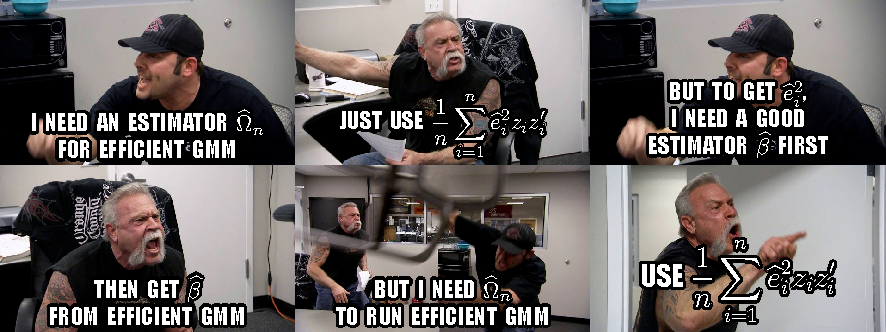
\includegraphics[width=0.85\linewidth]{figures/efficient-gmm.pdf}
	\caption{\emph{Well, at least we agree on weighting by $\widehat\Omega_n\inv$.}}
	\label{fig-meme}
\end{figure}

The way out is that \emph{any} consistent preliminary estimator gives a consistent $\widehat\Omega_n$,
and an inefficient \gls{gmm} estimator is still consistent.
We can first compute a preliminary estimator and get the residuals, then compute the efficient estimator.

\begin{definition}[Two-Step Feasible \glsentryshort{gmm}]
	The estimator is computed thus:
	\begin{enumerate}
		\item
			Compute a consistent preliminary estimator,
			such as $\widetilde\beta=\widehat\beta(S_{zz}\inv)=\widehat\beta_{\mathrm{2SLS}}$,
			and compute $\widehat\Omega_n$ from \eqref{eq-omega-hat} with the residuals $\widetilde e_i=y_i-x_i\T\widetilde\beta$.
		\item Compute $\widehat\beta(\widehat\Omega_n\inv)=(S_{zx}\T\widehat\Omega_n\inv S_{zx})\inv S_{zx}\T\widehat\Omega_n\inv s_{zy}$.
	\end{enumerate}
	Since $\widehat\Omega_n\inv\pto\Omega\inv$, \autoref{thm-efficient} applies and the estimator has optimal asymptotic variance $V^*$.
\end{definition}

\begin{remark}[Iterating]
	One can repeat the two steps until the estimate converges, which gives \emph{iterated} \gls{gmm}.
	It has the same asymptotic distribution as two-step \gls{gmm}, but it does not depend on the choice of preliminary estimator.
	A third option, \gls{cugmm}, lets the weighting matrix depend on $\beta$ inside the objective (\autoref{sec-cugmm}).
\end{remark}

\begin{remark}[Practical Concerns]\label{rmk-practical-concerns}
	$\widehat\Omega_n$ is $\ell\times\ell$ and has $\ell(\ell+1)/2$ distinct elements.
	With many moments it is estimated imprecisely, and because $\widehat\Omega_n$ is correlated with $\overline g_n$,
	efficient two-step \gls{gmm} can be badly biased in small samples \parencite{altonji-segal-1996}.
	Hence, in many cases, a simple fixed weight such as $W_n=S_{zz}\inv$ (i.e., \gls{tsls}) performs better in practice.
\end{remark}

\subsection{Homoskedasticity and \glsentryshort{tsls}}

\begin{proposition}[\glsentryshort{tsls} is Efficient \glsentryshort{gmm} under Homoskedasticity]
	Suppose, in addition to \autoref{ass-linear}, that $\E(e_i^2\given z_i)=\sigma^2$.
	Then $\Omega=\sigma^2\Sigma_{zz}$ with $\Sigma_{zz}=\E(z_iz_i\T)$, and \gls{tsls} is efficient \gls{gmm}.
\end{proposition}
\begin{proof}
	By the \gls{lie}, $\Omega=\E\bigl(\E(e_i^2\given z_i)z_iz_i\T\bigr)=\sigma^2\Sigma_{zz}$.
	The efficient weight $\Omega\inv=\sigma^{-2}\Sigma_{zz}\inv$ is a scalar multiple of $\Sigma_{zz}\inv$,
	and $S_{zz}\inv\pto\Sigma_{zz}\inv$.
	A scalar multiple of the weighting matrix does not change the estimator in \eqref{eq-gmm-explicit},
	so the efficient estimator can use $W_n=S_{zz}\inv$, which is \gls{tsls} by \autoref{ex-2sls}.
\end{proof}

\begin{remark}
	Without homoskedasticity, \gls{tsls} is still consistent and asymptotically normal by \autoref{thm-linear-asymptotics},
	but it is no longer efficient.
	Hence, the efficient \gls{gmm} estimator will generally differ from the \gls{tsls} estimator.
	Typically when doing feasible \gls{gmm}, people use \gls{tsls} as the preliminary estimator in two-step \gls{gmm}.
	Note that the usual caution about \gls{tsls} residuals still applies:
	$\widehat\Omega_n$ must be built from $\widetilde e_i=y_i-x_i\T\widetilde\beta$, not from the second-stage residuals $y_i-\widehat x_i\T\widetilde\beta$, where $\widehat x_i$ is the first-stage fitted value.
\end{remark}

\subsection{Testing Over-Identifying Restrictions}\label{sec-j-test}

When $\ell>k$, the sample moments cannot all be set to zero.
If all $\ell$ moment conditions hold, though, they should be close to zero at the efficient estimate.
This suggests evaluating the minimized objective.

\begin{theorem}[Hansen's $J$-Test]\label{thm-j-test}
	Under \autoref{ass-linear}, let $\widehat\Omega_n\pto\Omega$ and $\widehat\beta=\widehat\beta(\widehat\Omega_n\inv)$. Then
	\begin{align}
		J_n=J_n\bigl(\widehat\beta,\widehat\Omega_n\inv\bigr)=n\,\overline g_n(\widehat\beta)\T\widehat\Omega_n\inv\overline g_n(\widehat\beta)\dto\chi^2_{\ell-k}.
	\end{align}
\end{theorem}
\begin{proof}
	Since $\overline g_n(\widehat\beta)=s_{zy}-S_{zx}\widehat\beta=\overline g_n-S_{zx}(\widehat\beta-\beta_0)$, \eqref{eq-sampling-error} gives the exact identity
	\begin{align*}
		\overline g_n(\widehat\beta)=\bigl[I_\ell-S_{zx}(S_{zx}\T\widehat\Omega_n\inv S_{zx})\inv S_{zx}\T\widehat\Omega_n\inv\bigr]\overline g_n.
	\end{align*}
	Let $\widehat A=\widehat\Omega_n^{-1/2}S_{zx}$ and $\widehat P=\widehat A(\widehat A\T\widehat A)\inv\widehat A\T$.
	Multiplying by $\sqrt n\,\widehat\Omega_n^{-1/2}$,
	\begin{align*}
		\sqrt n\,\widehat\Omega_n^{-1/2}\overline g_n(\widehat\beta)=(I_\ell-\widehat P)\,v_n,
		\qquad
		v_n=\sqrt n\,\widehat\Omega_n^{-1/2}\overline g_n\dto\normaldistribution(0,I_\ell).
	\end{align*}
	Hence $J_n=v_n\T(I_\ell-\widehat P)v_n$.
	$\widehat P$ converges to $P=A(A\T A)\inv A\T$ with $A=\Omega^{-1/2}\Sigma_{zx}$,
	and $I_\ell-P$ is symmetric idempotent with rank $\ell-k$.
	So $J_n\dto\chi^2_{\ell-k}$.
\end{proof}

\begin{remark}[Why $\ell-k$ Degrees of Freedom]
	Estimating $k$ parameters sets $k$ linear combinations of the sample moments to zero,
	which is the first-order condition $S_{zx}\T\widehat\Omega_n\inv\overline g_n(\widehat\beta)=0$.
	Only the remaining $\ell-k$ directions carry information about whether the moment conditions hold.
	If $\ell=k$, then $J_n=0$ and there is nothing to test.
\end{remark}

\begin{remark}
	A few points are worth keeping in mind about the $J$-test:
	\begin{itemize}
		\item
			The null hypothesis is that \emph{all} $\ell$ moment conditions hold.
			Rejection says that some assumption fails, but not which one or which instrument.
			On the other hand, non-rejection is not proof of validity; the test may have low power.
		\item
			The $\chi^2_{\ell-k}$ limit requires the efficient weight $\widehat\Omega_n\inv$.
			With another weight, $J_n$ has a different limit.
		\item
			Under homoskedasticity, with $\widehat\Omega_n=\widehat\sigma^2S_{zz}$ and $\widehat\sigma^2=\widehat e\T\widehat e/n$,
			$J_n=\widehat e\T P_Z\widehat e/\widehat\sigma^2$ is the statistic of \textcite{sargan-1958},
			computed from the \gls{tsls} residuals.
			Hence, the $J$-test is also known as the Sargan-Hansen $J$-test.
	\end{itemize}
\end{remark}

\section{General \glsentryshort{gmm}: What Changes?}\label{sec-general-gmm}

The general problem replaces the linear moment function $z_i(y_i-x_i\T\beta)$ by any known function $g(w_i,\theta)$.
Let $\theta\in\Theta\subseteq\reals^k$ and $g(w_i,\theta)\in\reals^\ell$ satisfy
\begin{align}
	\E g(w_i,\theta_0)=0.
\end{align}
Define the sample and population moments and their Jacobians,
\begin{align*}
	g(\theta) &= \E g(w_i,\theta)\in\reals^{\ell}, &
	G(\theta) &= \frac{\partial g(\theta)}{\partial\theta\T}\in\reals^{\ell\times k},  \\
	\overline g_n(\theta) &= \frac1n\sum_{i=1}^ng(w_i,\theta)\in\reals^{\ell}, &
	G_n(\theta) &= \frac{\partial\overline g_n(\theta)}{\partial\theta\T}\in\reals^{\ell\times k}.
\end{align*}
The \gls{gmm} estimator is still defined as
\begin{align}\label{eq-general-gmm}
	\widehat\theta=\arg\min_{\theta\in\Theta} Q_n(\theta,W_n)
	\quad\text{where}\quad
	Q_n(\theta,W_n) = \overline g_n(\theta)\T W_n\overline g_n(\theta),
\end{align}
but in general it has no closed form solution.

\begin{remark}[$Q_n$ versus $J_n$]
	We write $Q_n$ for the unscaled objective and $J_n=n\,Q_n$ for the objective scaled by $n$, as in \eqref{eq-gmm-objective}.
	Scaling by $n$ does not change the minimizer, so either defines the same estimator.
	The two scalings serve different purposes:
	$Q_n(\theta,W_n)$ converges to the population objective $Q(\theta,W)=g(\theta)\T Wg(\theta)$, which is what consistency needs,
	while $J_n$ evaluated at the efficient estimate has a $\chi^2$ limit, which is what the $J$-test needs.
\end{remark}

\begin{remark}[Linear Model as a Special Case]
	The linear model is the special case $g(w_i,\beta)\coloneqq z_i(y_i-x_i\T\beta)$, for which
	\begin{align}\label{eq-linear-jacobian}
		G_n(\beta)=-S_{zx}
		\quad\text{and}\quad
		G(\beta)=-\Sigma_{zx}
	\end{align}
	for every $\beta$.
	Difference between the linear and general cases of \gls{gmm} comes from the fact that
	$G_n(\theta)$ depends on $\theta$ in general.
\end{remark}

\begin{remark}[Identification]
	In the linear model, the rank condition did two jobs.
	It made $\beta_0$ the unique root of the population moments, and it made $\Sigma_{zx}\T W\Sigma_{zx}$ invertible in the asymptotic variance.
	In general, these are separate conditions:
	\begin{itemize}
		\item \emph{Global identification:} $g(\theta)=0$ if and only if $\theta=\theta_0$. This is what consistency needs.
		\item \emph{Local identification:} $G_0=G(\theta_0)$ has full column rank $k$. This is what asymptotic normality needs.
		It is called \emph{local} because, near $\theta_0$, $g(\theta)\approx G_0(\theta-\theta_0)$,
		so full rank guarantees that $\theta_0$ is the only root of $g$ in a small neighborhood of $\theta_0$,
		but it says nothing about roots far away.
	\end{itemize}
	By \eqref{eq-linear-jacobian}, both reduce to the rank condition on $\Sigma_{zx}$ in the linear case.
	With nonlinear moments, neither implies the other in general.
\end{remark}

\subsection{Consistency}

Without a closed form solution, consistency must come from the properties of the sample and asymptotic objective function.

\begin{theorem}[Consistency]\label{thm-consistency}
	Assume the following:
	\begin{enumerate}
		\item Compactness: $\Theta$ is compact and contains $\theta_0$;
		\item Continuity: $g(\theta)$ is continuous;
		\item Global identification: $g(\theta)=0$ only at $\theta_0$;
		\item \gls{ulln}: $\sup_{\theta\in\Theta}\|\overline g_n(\theta)-g(\theta)\|\pto0$;
		\item Positive definite weights: $W_n\pto W$, which is positive definite.
	\end{enumerate}
	Then $\widehat\theta\pto\theta_0$.
\end{theorem}
\begin{proof}[Proof Sketch]
	Write $Q(\theta)=g(\theta)\T Wg(\theta)$ for the population objective.
	The \gls{ulln}, $W_n\pto W$, and boundedness of $g$ on the compact $\Theta$ give $\sup_{\theta\in\Theta}|Q_n(\theta,W_n)-Q(\theta)|\pto0$.
	By global identification and positive definiteness of $W$, $Q(\theta)>0=Q(\theta_0)$ for $\theta\ne\theta_0$,
	and by continuity and compactness, $\min_{\|\theta-\theta_0\|\ge\varepsilon}Q(\theta)>0$ for every $\varepsilon>0$.
	So any $\theta$ far from $\theta_0$ has an objective bounded away from the minimum,
	and once $Q_n$ is uniformly close to $Q$, the minimizer $\widehat\theta$ of $Q_n$ must lie within $\varepsilon$ of $\theta_0$ with probability approaching one.
	For a detailed proof, see \textcite{newey-mcfadden-1994} in the \emph{Handbook of Econometrics}.
\end{proof}

\begin{remark}[Interpretation of the Assumptions]
	The \gls{ulln} replaces the pointwise \gls{wlln}.
	Pointwise convergence at each $\theta$ is not enough, because $\widehat\theta$ is itself random:
	$Q_n$ could be close to $Q$ at every fixed $\theta$ and still have its minimum far from $\theta_0$.
	In the linear case, the explicit formula made this unnecessary.
\end{remark}

\subsection{Asymptotic Normality}

\begin{table}[t]
	\centering
	\caption{Linear versus general \gls{gmm}.}
	\label{tab-linear-general}
	\begin{tabular}{llp{0.42\linewidth}}
		\toprule
		& Linear                              & General                                       \\
		\midrule
		Estimator           & Closed form \eqref{eq-gmm-explicit} & Numerical minimization                        \\
		Identification      & Rank of $\Sigma_{zx}$               & Unique root of $g(\theta)$, and rank of $G_0$ \\
		Consistency         & \gls{wlln}                          & Compactness and \gls{ulln}                    \\
		Sampling error      & Exact \eqref{eq-sampling-error}     & Expansion \eqref{eq-expansion}                \\
		Asymptotic variance & $\Sigma_{zx}$ in \eqref{eq-avar}    & $G_0$ in place of $\Sigma_{zx}$               \\
		Efficient weight    & $\Omega\inv$                        & $\Omega\inv$                                  \\
		\bottomrule
	\end{tabular}
\end{table}

The first-order condition is $G_n(\widehat\theta)\T W_n\overline g_n(\widehat\theta)=0$.
In the linear case, the sampling error followed directly from it.
In general, $\overline g_n(\widehat\theta)$ must first be linearized around $\theta_0$.
By the fundamental theorem of calculus, applied along the segment from $\theta_0$ to $\widehat\theta$,
\begin{align}\label{eq-expansion}
	\overline g_n(\widehat\theta)=\overline g_n(\theta_0)+\widetilde G_n(\widehat\theta-\theta_0)
	\quad\text{where}\quad
	\widetilde G_n=\int_0^1G_n\bigl(\theta_0+t(\widehat\theta-\theta_0)\bigr)\diff t.
\end{align}
The integral form is used because the mean value theorem does not hold for vector-valued functions with a single intermediate point.
Substituting \eqref{eq-expansion} into the first-order condition and solving,
\begin{align}\label{eq-general-error}
	\sqrt n(\widehat\theta-\theta_0)
	=-\bigl(G_n(\widehat\theta)\T W_n\widetilde G_n\bigr)\inv G_n(\widehat\theta)\T W_n\sqrt n\,\overline g_n(\theta_0).
\end{align}

\begin{remark}[Compare with Linear Case]
	Compare this with \eqref{eq-sampling-error}: by \eqref{eq-linear-jacobian}, $G_n(\widehat\theta)=\widetilde G_n=-S_{zx}$ in the linear case, and the two coincide.
\end{remark}

\begin{theorem}[Asymptotic Normality]\label{thm-general-normality}
	In addition to the conditions of \autoref{thm-consistency}, suppose the following:
	\begin{enumerate}
		\item
			$\theta_0$ is in the interior of $\Theta$;
		\item
			$g(w,\theta)$ is continuously differentiable in $\theta$ on a neighborhood $U$ of $\theta_0$;
		\item
			\gls{ulln} in $G_n$: $\sup_{\theta\in U}\|G_n(\theta)-G(\theta)\|\pto0$;
		\item
			$G_0\coloneqq G(\theta_0)$ has full column rank $k$;
		\item
			\gls{clt}: $\sqrt n\,\overline g_n(\theta_0)\dto\normaldistribution(0,\Omega)$ with $\Omega=\E g(w_i,\theta_0)g(w_i,\theta_0)\T$.
	\end{enumerate}
	Then
	\begin{gather}
		\sqrt n(\widehat\theta-\theta_0)\dto\normaldistribution\bigl(0,V(W)\bigr)
		\shortintertext{where}
		V(W)=(G_0\T WG_0)\inv G_0\T W\,\Omega\,WG_0(G_0\T WG_0)\inv.
	\end{gather}
\end{theorem}
\begin{proof}[Proof Sketch]
	By consistency, with probability approaching one the segment from $\theta_0$ to $\widehat\theta$ lies in $U$.
	Uniform convergence of $G_n$ and continuity of $G$ then give $G_n(\widehat\theta)\pto G_0$ and $\widetilde G_n\pto G_0$.
	The rank condition makes $G_0\T WG_0$ invertible, and Slutsky's theorem applied to \eqref{eq-general-error} gives the result.
	The sign in \eqref{eq-general-error} does not affect the variance.
\end{proof}

\begin{remark}[Everything carries over from linear to general \gls{gmm}]
	$V(W)$ has exactly the form \eqref{eq-avar}, with $-G_0$ in place of $\Sigma_{zx}$.
	As a result, the rest of the linear theory carries over word for word, with $\Sigma_{zx}$ replaced by $G_0$ and $S_{zx}$ by $G_n(\widehat\theta)$:
	\begin{itemize}
		\item The efficient weight is $W=\Omega\inv$, with $V^*=(G_0\T\Omega\inv G_0)\inv$, by the same proof as \autoref{thm-efficient}.
		\item If $\ell=k$, then $V(W)=G_0\inv\Omega(G_0\T)\inv$ for every $W$.
		\item Two-step efficient \gls{gmm} uses $\widehat\Omega_n=n\inv\sum_ig(w_i,\widetilde\theta)g(w_i,\widetilde\theta)\T$ from a preliminary $\widetilde\theta$.
			The standard errors use $\widehat V^*=(\widehat G\T\widehat\Omega_n\inv\widehat G)\inv$ with $\widehat G=G_n(\widehat\theta)$.
		\item The $J$-test still has a $\chi^2_{\ell-k}$ limit. The identity in the proof of \autoref{thm-j-test} now holds up to an $o_p(1)$ term.
	\end{itemize}
	A comparison of the linear and general cases is summarized in \autoref{tab-linear-general}.
\end{remark}

\begin{remark}[A Practical Point]
	$\widehat V$ must correspond to the weight used.
	For a general $W_n$, use the sandwich $\widehat V=(\widehat G\T W_n\widehat G)\inv\widehat G\T W_n\widehat\Omega_nW_n\widehat G(\widehat G\T W_n\widehat G)\inv$ with $\widehat G=G_n(\widehat\theta)$.
	Only for efficient \gls{gmm} does it simplify to $\widehat V^*=(\widehat G\T\widehat\Omega_n\inv\widehat G)\inv$.
\end{remark}

\begin{remark}[A \gls{lr} Relation]
	With the efficient weight, there is also an analogue of the \gls{lr} test:
	if $\widetilde\theta$ minimizes $J_n(\theta,\widehat\Omega_n\inv)$ subject to $r(\theta)=0$, then
	$J_n(\widetilde\theta,\widehat\Omega_n\inv)-J_n(\widehat\theta,\widehat\Omega_n\inv)\dto\chi^2_q$ under $H_0$,
	provided the same $\widehat\Omega_n$ is used in both objectives \parencite[Chapter 3]{hayashi-2000}.
\end{remark}

\section{Extensions and Related Topics}

\subsection{Conditional Moments and Optimal Instruments}

Economic models often imply a \emph{conditional} moment restriction, such as $\E(e_i\given z_i)=0$ in $y_i=x_i\T\beta_0+e_i$.
This is much stronger than $\E(z_ie_i)=0$:
for any vector-valued function $h(z_i)$ with finite moments, the \gls{lie} gives
\begin{align}
	\E[h(z_i)e_i]=\E[h(z_i)\E(e_i\given z_i)]=0.
\end{align}
So every choice of $h$ yields valid unconditional moments $g(w_i,\beta)=h(z_i)(y_i-x_i\T\beta)$,
for example $h(z_i)=(1,z_i,z_i^2,\ldots,z_i^L)\T$ for scalar $z_i$.

\begin{remark}[The Many-Moments Problem]
	Asymptotically, adding valid moments never increases the variance of efficient \gls{gmm}.
	In finite samples, however, more moments are not automatically better.
	When the number of instruments grows with the sample size, $\ell/n\to\alpha>0$,
	\gls{tsls} is inconsistent,
	and two-step efficient \gls{gmm} suffers from the same many-moments bias.
\end{remark}

\begin{theorem}[Optimal Instrument]\label{thm-optimal-instrument}
	Suppose $y_i=x_i\T\beta_0+e_i$ with $\E(e_i\given z_i)=0$ and write $\sigma^2(z_i)=\E(e_i^2\given z_i)>0$.
	Let $h(z_i)\in\reals^k$ denote instrument functions with $\E(h(z_i)x_i\T)$ invertible.
	Let $g_i(\beta)\coloneqq h(z_i)(y_i-x_i\T\beta)$ and $\widehat\beta_h$ be the solution to the \gls{gmm} problem.
	Then, its asymptotic variance is
	\begin{align}
		V(h)=\bigl[\E(h(z_i)x_i\T)\bigr]\inv\E\bigl[\sigma^2(z_i)h(z_i)h(z_i)\T\bigr]\bigl[\E(x_ih(z_i)\T)\bigr]\inv,
	\end{align}
	and it is minimized by the optimal instrument of \textcite{chamberlain-1987},
	\begin{align}
		h^*(z_i)=\frac{\E(x_i\given z_i)}{\E(e_i^2\given z_i)}.
		% \qquad
		% V^*=V_{h^*}=\left[\E\left(\frac{D(z_i)D(z_i)\T}{\sigma^2(z_i)}\right)\right]\inv.
	\end{align}
	That is, $V(h)-V(h^*)$ is positive semidefinite for every $h$.
\end{theorem}
\begin{proof}
	The formula for $V(h)$ is just \autoref{thm-linear-asymptotics} with instruments $h(z_i)$,
	where the middle term $\E\bigl(e_i^2h(z_i)h(z_i)\T\bigr)$ equals $\E\bigl(\sigma^2(z_i)h(z_i)h(z_i)\T\bigr)$ by the \gls{lie}.
	By the \gls{lie} again, for every $h$,
	\begin{align*}
		\E\bigl(\sigma^2(z_i)h(z_i)h^*(z_i)\T\bigr)
		=\E\bigl(h(z_i)\E(x_i\given z_i)\T\bigr)
		=\E\bigl(h(z_i)x_i\T\bigr).
	\end{align*}
	Taking $h=h^*$ shows that $\E(h^*(z_i)x_i\T)=\E(\sigma^2(z_i)h^*(z_i)h^*(z_i)\T)$ is symmetric, so $V(h^*)=\bigl[\E\bigl(\sigma^2(z_i)h^*(z_i)h^*(z_i)\T\bigr)\bigr]\inv$.
	Now consider the variance of the difference
	\begin{align*}
		\bigl[\E(h(z_i)x_i\T)\bigr]\inv h(z_i)e_i-V(h^*)h^*(z_i)e_i.
	\end{align*}
	The first term has variance $V(h)$, and the second has variance $V(h^*)$.
	Their covariance is
	\begin{align*}
		\bigl[\E(h(z_i)x_i\T)\bigr]\inv\E\bigl(\sigma^2(z_i)h(z_i)h^*(z_i)\T\bigr)V(h^*)
		&=\bigl[\E(h(z_i)x_i\T)\bigr]\inv\E\bigl(h(z_i)x_i\T\bigr)V(h^*) \\
		&=V(h^*).
	\end{align*}
	Therefore, the variance of the difference is $V(h)-2V(h^*)+V(h^*)=V(h)-V(h^*)$, which is positive semidefinite.
\end{proof}

\begin{remark}[Intuition]
	The optimal instrument has two parts: the numerator $\E(x_i\given z_i)$ and the denominator $\E(e_i^2\given z_i)$.
	\begin{itemize}
		\item
			The numerator $\E(x_i\given z_i)$ is the best prediction of $x_i$ from $z_i$:
			it keeps exactly the part of $x_i$ that the instruments can explain, which is all the information $z_i$ carries about $\beta_0$.
		\item
			The denominator $\E(e_i^2\given z_i)$ down-weights observations with noisy errors, as in \gls{gls}.
	\end{itemize}
	Since $h^*$ has $k$ components, the optimal moments are exactly identified:
	any number of candidate moments is reduced to the $k$ best combinations.
	The result also covers over-identified \gls{gmm} with moments $H(z_i)e_i$ for any finite set of functions $H$,
	because efficient \gls{gmm} with those moments is equivalent to using the $k$ instruments $G_0\T\Omega\inv H(z_i)$.
\end{remark}

\begin{remark}[Relation to \glsentryshort{wls}]
	If $x_i$ is exogenous, we can take $z_i=x_i$.
	Then $\E(x_i\given x_i)=x_i$ and $h^*(x_i)=x_i/\sigma^2(x_i)$,
	so $\widehat\beta_{h^*}$ solves $\sum_ix_i(y_i-x_i\T\beta)/\sigma^2(x_i)=0$.
	This is \gls{wls} with weights $1/\sigma^2(x_i)$.
	Hence \gls{wls} is the efficient estimator under $\E(e_i\given x_i)=0$,
	and with homoskedastic errors it reduces to \gls{ols}.
\end{remark}

\begin{remark}[Relation to \glsentryshort{tsls}]
	Under conditional homoskedasticity, $\sigma^2(z_i)=\sigma^2$ is constant, so $h^*(z_i)$ is proportional to $\E(x_i\given z_i)$.
	If, in addition, the first stage is linear, $\E(x_i\given z_i)=\Pi\T z_i$,
	then using the instruments $\widehat\Pi\T z_i$, with $\widehat\Pi$ from the first-stage regression, gives \gls{tsls}.
	So, with homoskedastic errors and a linear first stage, \gls{tsls} is efficient among \emph{all} instruments built from $z_i$,
	not only among those linear in $z_i$.
\end{remark}

\begin{remark}[In Practice]
	Both $\E(x_i\given z_i)$ and $\E(e_i^2\given z_i)$ are unknown functions of $z_i$,
	so they must be estimated, typically by nonparametric methods.
	Estimating them well requires large samples, and in finite samples the estimation error can offset the efficiency gain.
	If feasible two-step \gls{gmm} is already difficult to compute (\autoref{rmk-practical-concerns}),
	then estimating the optimal instruments is even more so.
	This is one reason optimal instruments are rarely used in applied work,
	where a moderate number of instruments with efficient \gls{gmm} is more common.
\end{remark}

\subsection{Dependent Data and \glsentryshort{hac} Estimation}\label{sec-hac}

With time series data, the observations are not independent, and $g_i=g(w_i,\theta_0)$ may be serially correlated.
Under stationarity and weak dependence, the moments still satisfy a \gls{clt}, but the asymptotic variance changes to the \emph{long-run covariance}
\begin{align}
	\Omega=\sum_{j=-\infty}^{\infty}\Gamma_j,
	\quad\text{where}\quad
	\Gamma_j=\E g_ig_{i-j}\T.
\end{align}
Everything about \gls{gmm} still holds with this $\Omega$,
including the efficient weight $\Omega\inv$ and the $J$-test.
What changes is that we need a \gls{hac} estimator of $\Omega$:
\begin{align}
	\widehat\Omega_{\mathrm{HAC}}=\widehat\Gamma_0+\sum_{j=1}^Lk(j,L)\bigl(\widehat\Gamma_j+\widehat\Gamma_j\T\bigr)
	\quad\text{where}\quad
	\widehat\Gamma_j=\frac1n\sum_{i=j+1}^n\widehat g_i\widehat g_{i-j}\T,
\end{align}
for a kernel $k$ and bandwidth $L$.
Our trusty old \textcite{newey-west-1987} with Bartlett kernel guarantees that $\widehat\Omega_{\mathrm{HAC}}$ is positive semidefinite.

\subsection{Continuously Updated \glsentryshort{gmm} and \glsentryshort{liml}}\label{sec-cugmm}

Two-step \gls{gmm} fixes the weighting matrix at a preliminary estimate.
\gls{cugmm} \parencite{hansen-heaton-yaron-1996} instead lets the weight vary with $\theta$ inside the objective:
\begin{align}
	\widehat\theta_{\mathrm{CU}}=\arg\min_{\theta\in\Theta}\overline g_n(\theta)\T\widehat\Omega_n(\theta)\inv\overline g_n(\theta)
	\quad\text{where}\quad
	\widehat\Omega_n(\theta)=\frac1n\sum_{i=1}^ng(w_i,\theta)g(w_i,\theta)\T.
\end{align}
It has the same asymptotic distribution as efficient two-step \gls{gmm}.
In finite samples, \textcite{hansen-heaton-yaron-1996} find that it is less biased than two-step \gls{gmm} but has fatter tails.
This is consistent with the example below: in the linear homoskedastic model it reduces to \gls{liml}, which has no finite moments.
It typically requires numerical optimization, and the objective is not convex in general,
so it is more difficult to compute than two-step \gls{gmm}.
Its advantage is that it does not depend on a preliminary estimator.

\begin{example}[\glsentryshort{cugmm} in the Linear Model]\label{ex-cugmm-liml}
	In the linear \gls{iv} model with $u(\beta)=y-X\beta$, suppose the weight is computed under homoskedasticity,
	\begin{align*}
		\widehat\Omega_n(\beta)=\frac{u(\beta)\T u(\beta)}{n}\cdot\frac{Z\T Z}{n}.
	\end{align*}
	Then the continuously updated objective, scaled by $n$, is
	\begin{align*}
		J_n(\beta)
		=n\left(\frac{Z\T u(\beta)}{n}\right)\T\left(\frac{u(\beta)\T u(\beta)}{n}\cdot\frac{Z\T Z}{n}\right)\inv\frac{Z\T u(\beta)}{n}
		=n\,\frac{u(\beta)\T P_Zu(\beta)}{u(\beta)\T u(\beta)}.
	\end{align*}
	Since $u\T u=u\T P_Zu+u\T M_Zu$ with $M_Z=I_n-P_Z$,
	\begin{align*}
		\frac{u\T P_Zu}{u\T u}=1-\frac{u\T M_Zu}{u\T u},
	\end{align*}
	so minimizing $J_n(\beta)$ is the same as minimizing $u(\beta)\T u(\beta)/u(\beta)\T M_Zu(\beta)$.
	This is the \gls{liml} criterion, when there are no included exogenous regressors.
	With included exogenous regressors, they are first partialled out.
	So, under homoskedasticity, \gls{liml} is continuously updated \gls{gmm},
	in the same way that \gls{tsls} is efficient two-step \gls{gmm}.
\end{example}

\begin{remark}[Exactly \glsentryshort{liml}]
	With the homoskedastic weight in \autoref{ex-cugmm-liml}, \gls{cugmm} and \gls{liml} give numerically identical estimates in every sample, not just asymptotically equivalent ones.
	With the heteroskedasticity-robust weight $\widehat\Omega_n(\beta)=n\inv\sum_iu_i(\beta)^2z_iz_i\T$, however,
	the objective is no longer a ratio of two quadratic forms, and \gls{cugmm} differs from \gls{liml} in finite samples.
\end{remark}

\vfill
\section*{Acronyms}
\printglossaries

{\sloppy\printbibliography[heading=bibintoc,title={References}]}

\end{document}
